\section{Grasp Envelope Extraction}
\label{sec:method}
%%%%%%%%%%%%%%%%%%%%%%%%%%%%%%%%%%%%%%%%%%%%%%%%%%%%%%%%%%%%%%%%%%%%%%%%%%%%%%%%%%%%%%%%%%%%%%%%%%%%%%%%%%%%%%%%%%%%%%%
\begin{figure}[t!]
\centering
\subfigure[] {
        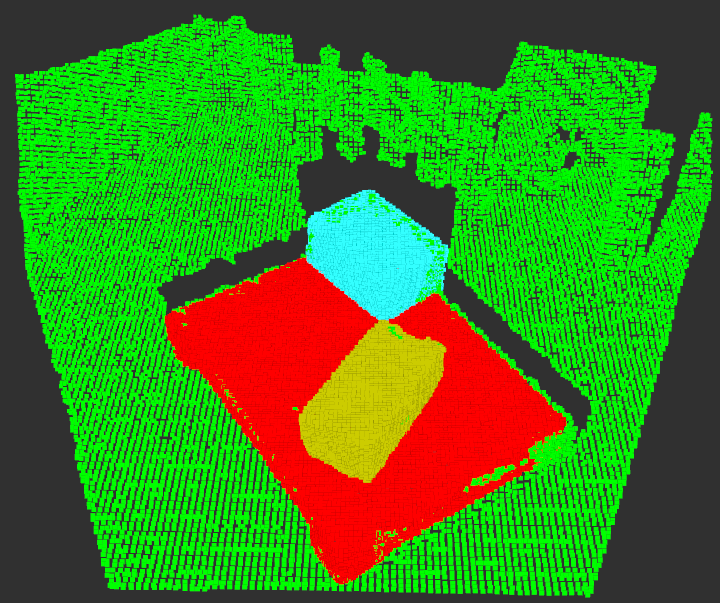
\includegraphics[width = 0.46\linewidth, height=3.5cm]{figs/primitive.png}
	\label{fig:grasp_primitive}
}
\subfigure[] {
        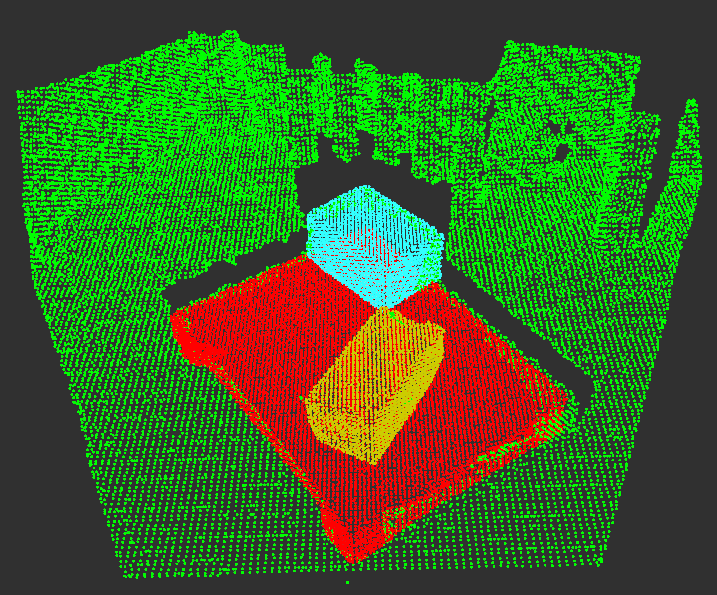
\includegraphics[width = 0.46\linewidth, height=3.5cm]{figs/truncated_raster_axis}
	\label{fig:grasp_interval}
}
\caption{An illustration of a cylindrical grasp envelope primitive in~\subref{fig:grasp_primitive}
  and a corresponding grasp envelope in~\subref{fig:grasp_interval}. The constraints are satisfied
  for any end effector pose which brings the gripper reference frame inside the shaded cylindrical
  shell sector, while maintaining orientation of the $x$ and $z$ axis within their respective shaded
  cone regions.}
\label{fig:grasp_envelope}
\end{figure}
%%%%%%%%%%%%%%%%%%%%%%%%%%%%%%%%%%%%%%%%%%%%%%%%%%%%%%%%%%%%%%%%%%%%%%%%%%%%%%%%%%%%%%%%%%%%%%%%%%%%%%%%%%%%%%%%%%%%%%%
\subsection{Grasp Envelopes}
Let $\mbm{p} = \left[x,y,z,o_x,o_y,o_z,o_w\right]^T$ be the pose of the gripper frame relative to a fixed frame connected to the robot kinematic model, represented by a 3D translation and a quaternion-encoded orientation. 
In addition, let $\mbm{q} \in \mathbb{R}^n$ be the configuration vector describing the joint angles of all $n$ gripper joints.
We represent the posture of the gripper as a vector $ \mbm{x} = \left[\mbm{p}^T, \mbm{q}^T\right]^T$.
We then define a grasp envelope $\mathcal{G}$ as a set of gripper postures satisfying constraints imposed on the gripper pose and joint configuration:
\begin{equation}
\mathcal{G} = \left\{ \mbm{x} \in \mathbb{R}^{n+7} \,|\, c_i(\mbm{x}) \leq 0,\, i = 1, \ldots, m \right\}
\label{eq:constraints}
\end{equation}
%
In this work, we restrict our analysis to linear inequality constraints, in order to facilitate an efficient implementation.
In addition, we concentrate our analysis on an underactuated gripping device with a single actuated degree of freedom, thus $q \in \mathbb{R}$. 
For simplicity, we only impose box constraints on the gripper opening angle, $i. \, e.$, $q_{min} \leq q \leq q_{max}$.
\par
The definition of a grasp envelope $\mathcal{G}$ in~\eqref{eq:constraints} allows us to encode various constraints on the robot end effector pose.
In this work we define two prototypical sets of grasp envelope constraints, which we term \textit{grasp envelope primitives} --- a cylindrical and a spherical primitive.
At runtime, the algorithms in Sec.~\ref{sec:collision_check} and~\ref{sec:fitting_bb} are used to refine the bounds on these primitives and obtain valid collision-free grasp envelopes for a particular object placement in the workspace.

An illustration of a cylindrical grasp envelope primitive is shown in Fig.~\ref{fig:grasp_primitive}, while a grasp envelope obtained by imposing additional bounds\footnote{In previous work~\cite{Krug15} we refer to this as a \textit{truncated} grasp envelope.} on the primitive is shown in Fig.~\ref{fig:grasp_interval}. 

Our treatment of the spherical shell grasp primitive is done in an analogous manner, by constraining
the gripper pose in between two concentric spheres while aligning the gripper's approach axis with
the vector pointing towards the sphere center and maintaining the gripper's lateral axis ($y$ in
Fig.~\ref{fig:grasp_envelope}) approximately parallel to a horizontal plane. 
\par
%%%%%%%%%%%%%%%%%%%%%%%%%%%%%%%%%%%%%%%%%%%%%%%%%%%%%%%%%%%%%%%%%%%%%%%%%%%%%%%%%%%%%%%%%%%%%%%%%%%%%%%%%%%%%%%%%%%%%%%
\begin{figure*}[t!]
\centering
\subfigure[] {
        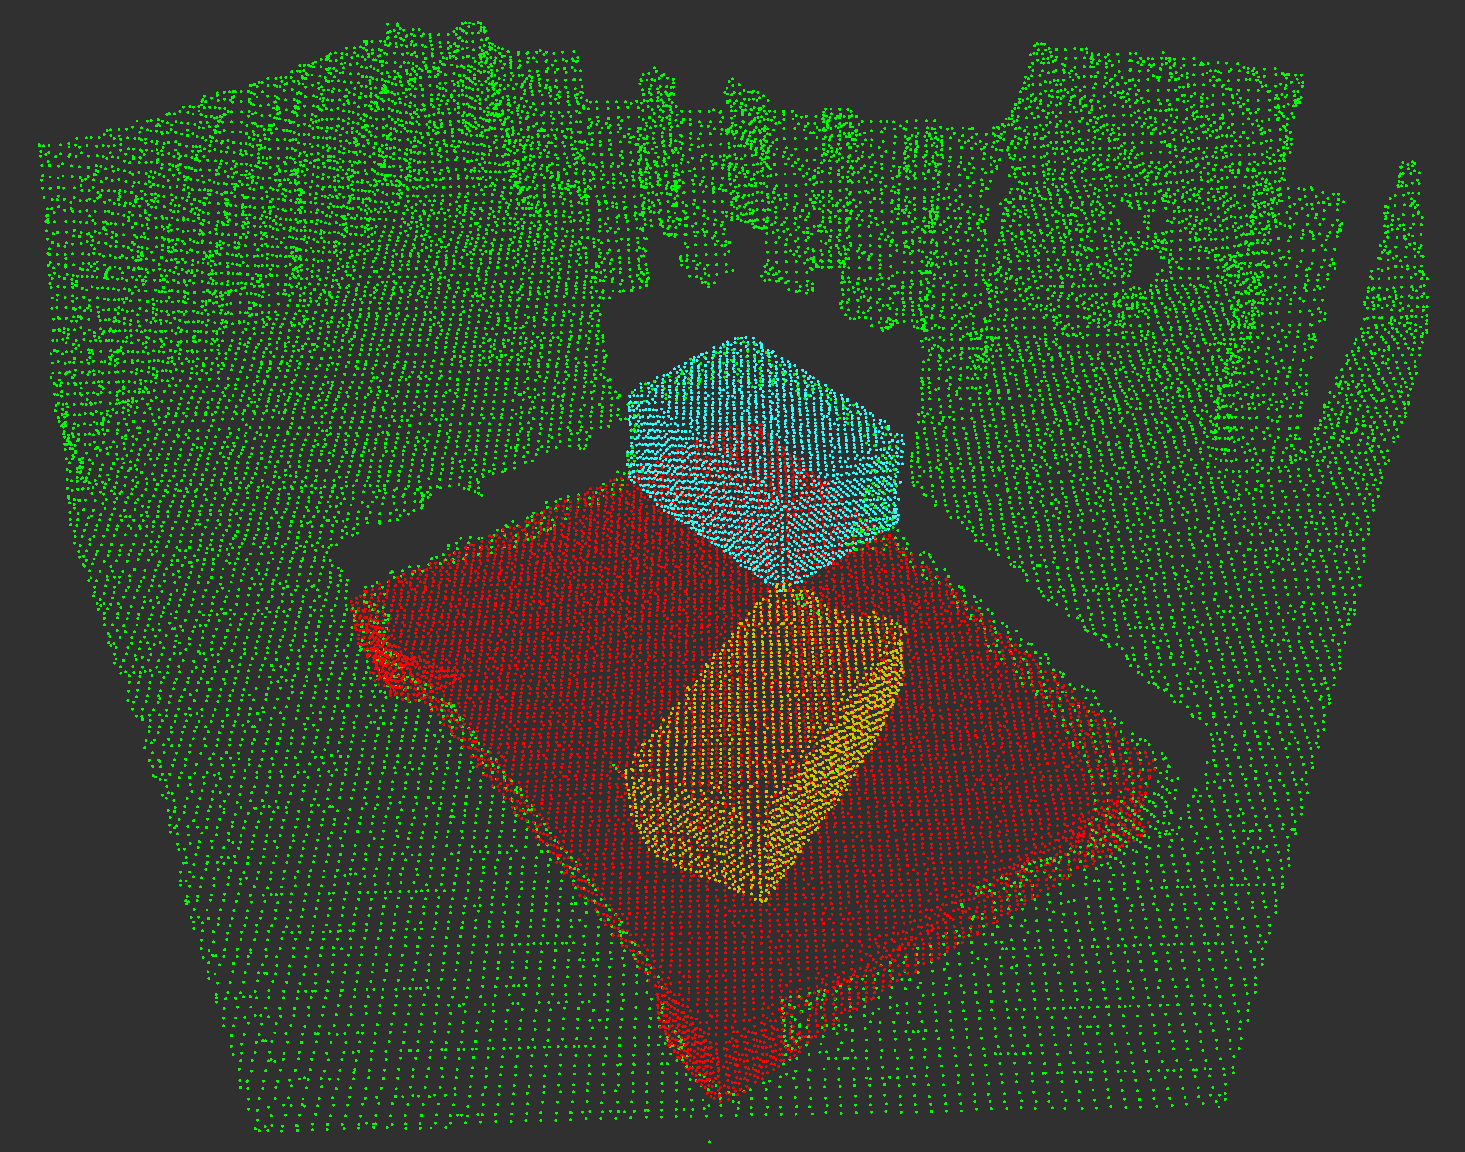
\includegraphics[width = .31\linewidth, height=5.0cm]{figs/collision_grid}
	    \label{fig:collision_grid}
}
\subfigure[] {
        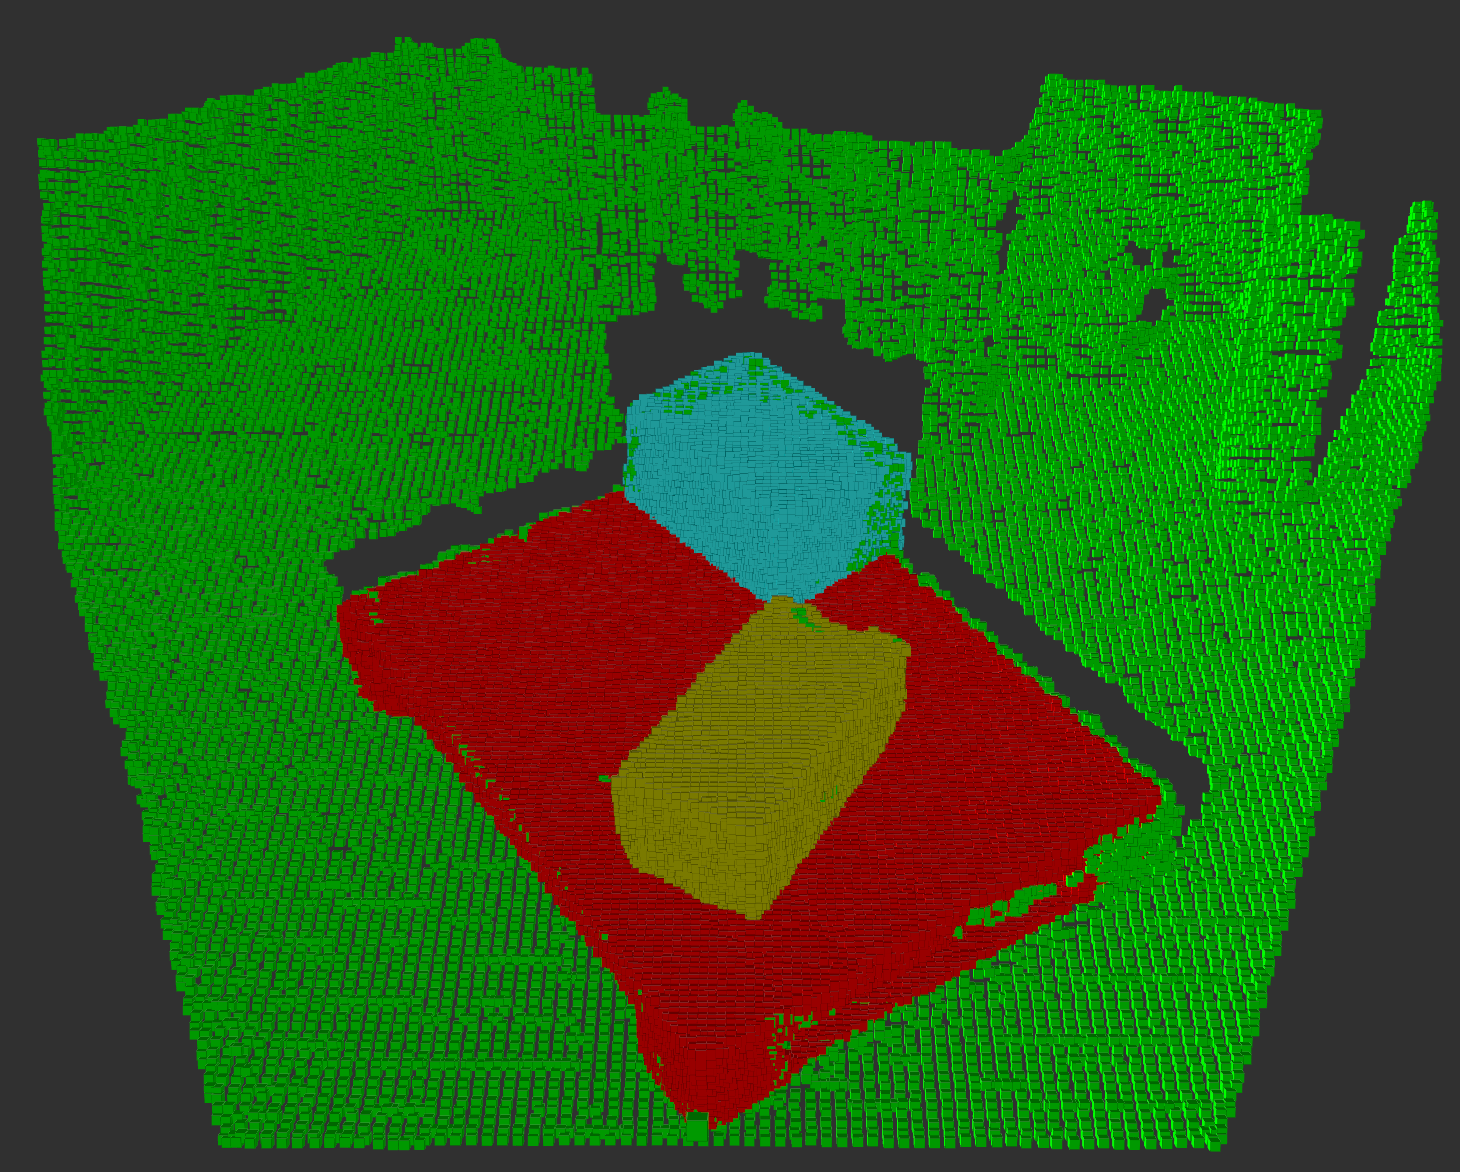
\includegraphics[width = .31\linewidth, height=5.0cm]{figs/valid_configs}
	    \label{fig:valid_configs}
}
\subfigure[] {
        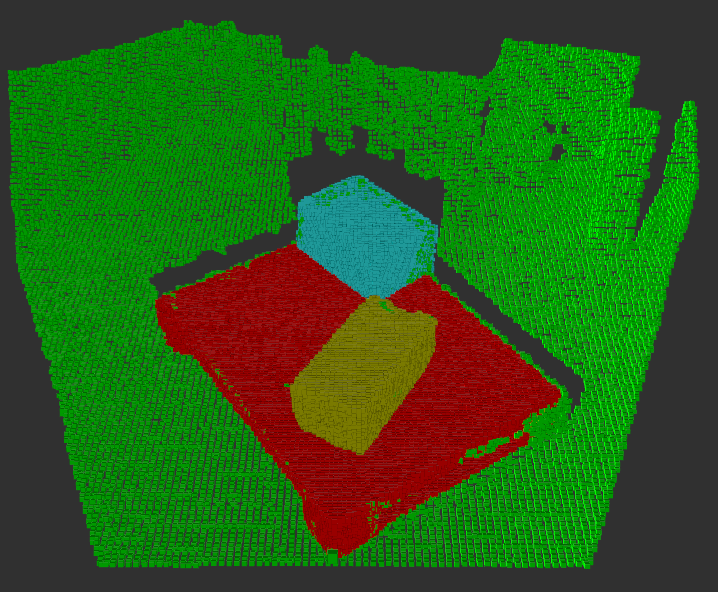
\includegraphics[width = .31\linewidth, height=5.0cm]{figs/distance_field}
	    \label{fig:distance_field}
}
\caption{Two-dimensional illustrations of the three main steps of our approach: \subref{fig:collision_grid} approach to pre-computing a collision map for the initial grasp envelope primitive; \subref{fig:valid_configs} three types of collisions which can occur and which are handled differently by our approach; \subref{fig:distance_field} process used for finding the maximum-volume cluster of valid grasp postures. The maximum-volume cluster in \subref{fig:distance_field} is shown in the shaded rectangle labeled \textbf{b}. }
\label{fig:method}
\end{figure*}
%%%%%%%%%%%%%%%%%%%%%%%%%%%%%%%%%%%%%%%%%%%%%%%%%%%%%%%%%%%%%%%%%%%%%%%%%%%%%%%%%%%%%%%%%%%%%%%%%%%%%%%%%%%%%%%%%%%%%%%
\subsection{Pre-computing a Collision Map}
\label{sec:sampling}
%
The first step of our approach is to pre-compute a 3D collision map for each of the two grasp envelope primitives.
This step is performed offline and greatly speeds up the subsequent online primitive refinement.
The procedure, illustrated by the 2D projection in Fig.~\ref{fig:collision_grid}, begins by sampling gripper poses from the initial envelope primitive.
We obtain the samples with a regular grid in the parametric space of each primitive and store them in a regular sample grid $\mathcal{S}$.
For the cylindrical shell primitive we sample along the distance to the center $d$, the orientation $\alpha$ (w.r.t. the cylinder  coordinate frame), and the height above the horizontal plane $h$. 
Similarly, the spherical shell primitive is parametrized by the radius $r$, and the polar and azimuth angles $\theta,\phi$.
\par
Next, for each sampled gripper pose we generate the gripper footprint in a collision map. 
As shown in Fig.~\ref{fig:collision_grid}, for this step we use an idealized gripper model, consisting of a bounding box around the palm and a semi-cylinder covering all possible placements of the fingers under different opening angles.
Each cell of the collision map covered by the ideal gripper footprint is then marked as occupied by the currently evaluated sample from $\mathcal{S}$. 
By iterating this procedure over all samples in $\mathcal{S}$ we obtain a collision map which encodes in every cell the list of gripper postures that would potentially occupy it.
%
%%%%%%%%%%%%%%%%%%%%%%%%%%%%%%%%%%%%%%%%%%%%%%%%%%%%%%%%%%%%%%%%%%%%%%%%%%%%%%%%%%%%%%%%%%%%%%%%%%%%%%%%%%%%%%%%%%%%%%%
\subsection{Finding Valid Configurations in Reconstructed Scenes}
\label{sec:collision_check}
Once we obtain the intersection between the two maps, we iterate through all affected cells in the collision map and check the affected gripper pose samples from $\mathcal{S}$.
As illustrated in Fig.~\ref{fig:valid_configs}, we distinguish between three types of collisions: 1) between the gripper palm and the map; 2) between the gripper fingers and the target object; and 3) between the fingers and other objects in the environment. 
Case 1) entails that the considered gripper pose would result in a collision, and thus we mark the corresponding sample in $\mathcal{S}$ as invalid.
Cases 2) and 3) would result in a collision only for specific configurations of the gripper opening angle $q$, thus we use them to impose tighter bounds on $q_{min}$ and $q_{max}$ associated with the respective sample in $\mathcal{S}$. 
At the end of this procedure we check the bounds on $q_{min},q_{max}$ for all remaining valid samples in $\mathcal{S}$ and invalidate those that impose infeasible constraints ($i.\,e.$, $q_{min}\geq q_{max}$) and those that would not result in a grasp of the target object ($q_{min} = 0$ when no contact with the object was detected).

\subsection{Fitting a Maximum Volume Envelope}
\label{sec:fitting_bb}
%
Following the procedures outlined in the previous subsections, we obtain a grid of discrete samples $\mathcal{S}$ representing a set of gripper postures.
Some of the postures in $\mathcal{S}$ have been invalidated by the collision checks in Sec.~\ref{sec:collision_check}, while the remaining ones are valid under certain bounds on $q$.
In order to obtain a refined grasp envelope following the definition in \eqref{eq:constraints}, we need to find a set of inequality constraints in Cartesian space containing only valid samples from $\mathcal{S}$. 
Thanks to our regular grid sampling strategy from Sec.~\ref{sec:sampling}, it is straightforward to obtain a set of Cartesian-space constraints for any axis-aligned bounding box in $\mathcal{S}$.
Thus, we can obtain a refined grasp envelope by looking for the largest axis-aligned inscribed box in $\mathcal{S}$: $i.\,e.$, the maximum volume box containing only valid samples.
\par
Finding maximum volume/area inscribed shapes is in general a hard problem.
Our problem instance is however additionally constrained to a regular sample grid and axis aligned shapes, and can therefore be solved efficiently.
If we treat invalid samples in $\mathcal{S}$ as occupied space, and conversely valid samples as free space, we can use a variant of the distance transform to speed up our search.
In general, we are looking for a $k$ dimensional axis-aligned bounding box, with $k$ being the dimensionality of the sampling grid $\mathcal{S}$. 
For simplicity, in this section we discuss a 2D version of our approach (illustrated in Fig.~\ref{fig:distance_field}), which is readily extendable to $k$D.
The main idea here is to look for the best position of the lower-right corner of the maximum bounding rectangle (the shaded rectangle labeled \textbf{b} in Fig.~\ref{fig:distance_field}).
We first construct a 2D distance field which for every free cell encodes the distance to the closest occupied cell in the negative direction ($i.\,e.$, towards the upper-left corner), along each dimension.
This provides us with an absolute upper bound on the volume of a box which uses a particular cell as a lower-right corner: $e.\,g.$, the example labeled \textbf{a} in Fig.~\ref{fig:distance_field} would result in a maximal volume of $8\times5=40$ samples.
Using this as a criterion to prune the search space, Algorithm~\ref{alg:bbsearch} can be used to find the maximal-area box. 
Lines 8-15 in the algorithm describe the search procedure along the $x$ direction of the distance grid, as shown also in case \textbf{b} of Fig.~\ref{fig:distance_field}.
In essence, we keep track of the maximum area rectangle verified so far ($m_i,m_j$), and update it for every slice along $x$ in lines 10-11. 
We next check if it is possible to obtain a larger area rectangle (in the best case) if we continue searching.
If so, we refine the boundary $d_j$ along $y$ (lines 12-13), otherwise we stop the search (line 15).
Last, we check if the rectangle obtained in this manner is larger than the current best candidate and move to the next possible bottom-right corner (lines 18-19).
For the envelope primitives discussed in this work, $k=3$ and we obtain a straight-forward extension of the presented algorithm to 3D by searching in addition along the third dimension.
At a moderate computational cost, this algorithm can be modified to extract the top $N$ largest volume regions. 
Finally, since the zero position for sampling dimensions associated with varying orientation is arbitrary, in these cases we allow regions to span across the first-to-last element border and modify the distance field computation accordingly.
\begin{algorithm}[t!]
\DontPrintSemicolon % Some LaTeX compilers require you to use \dontprintsemicolon instead 
\KwIn{Distance transform $D$}
$V_{max} \gets 0$\;
%\For{$x,y \gets 1$ \textbf{to} $|D|_x,|D|_y$}{
\For{$\forall$ cells in $D$}{
    Let $i,j \gets$ index of current cell, $D_{i,j}^x,D_{i,j}^y\gets$ value of $D$ at $i,j$ along $x,y$ dimensions \;
    \If{$(i-D_i)(j-D_j) > V_{max}$} {
	$m_i,m_j \gets 0$ \;
	$d_i,d_j \gets D_{i,j}^x,D_{i,j}^y$ \;    
	//search along $x$ \;
	\For{$k\gets i$ \textbf{to} $i-D_i$} {
	    $d_{min} \gets min(d_j,D_{k,j}^y)$ \;
	    \If{$(k-i) d_{min}> m_i m_j$ } {
		$m_i,m_j \gets k-i, d_{min}$ \;
	    }
	    \If{ $d_i d_{min} > m_i m_j$} {
		$d_j \gets d_{min}$ \;
	    }	
	    \Else {
		break \;
	    }
	}
	//search along $y$ equivalent \;
	$\ldots$ \;
	\If{$(i-m_i)(j-m_j) > V_{max}$} {
	    $V_{max} \gets (i-m_i)(j-m_j)$, store bounds \;
	}
    }
}
\Return{$V_{max}$, bounds}\;
\caption{{\sc BBSearch2D:} find largest rectangle}
\label{alg:bbsearch}
\end{algorithm}
